\section{EBeSS Design Methodology}	\label{sec:tech}
%
This section demonstrates the design methodology of EBeSS.
After introducing the overview of EBeSS structure, we illustrates the two key techniques embedded in the simulator.
\emph{Energy Message Handling (EMH) Framework} supports the energy behavior of each hardware modules and handles the energy messages according to power supply changes.
\emph{Virtual Device} supports the simulation of the peripherals.

\subsection{Structure Overview of EBeSS}		\label{sec:tech-structure}
%
EBeSS is an energy-aware system-level simulator designed based on GEM5 and NVPSim. 
EBeSS adopts the fundamental usage and logic of core architecture in GEM5 and the energy supply structure in NVPSim.
By developing two novel components, EBeSS enables the ability of simulating the energy behaviors of energy-aware systems, such as non-volatile processors, multi-frequency systems, or multi-voltage-domain systems. 
The system architecture of EBeSS is shown in Fig.~\ref{fig:techStructure}.

\begin{figure}[!htpb]
	\centering
	\vspace{-10pt}
	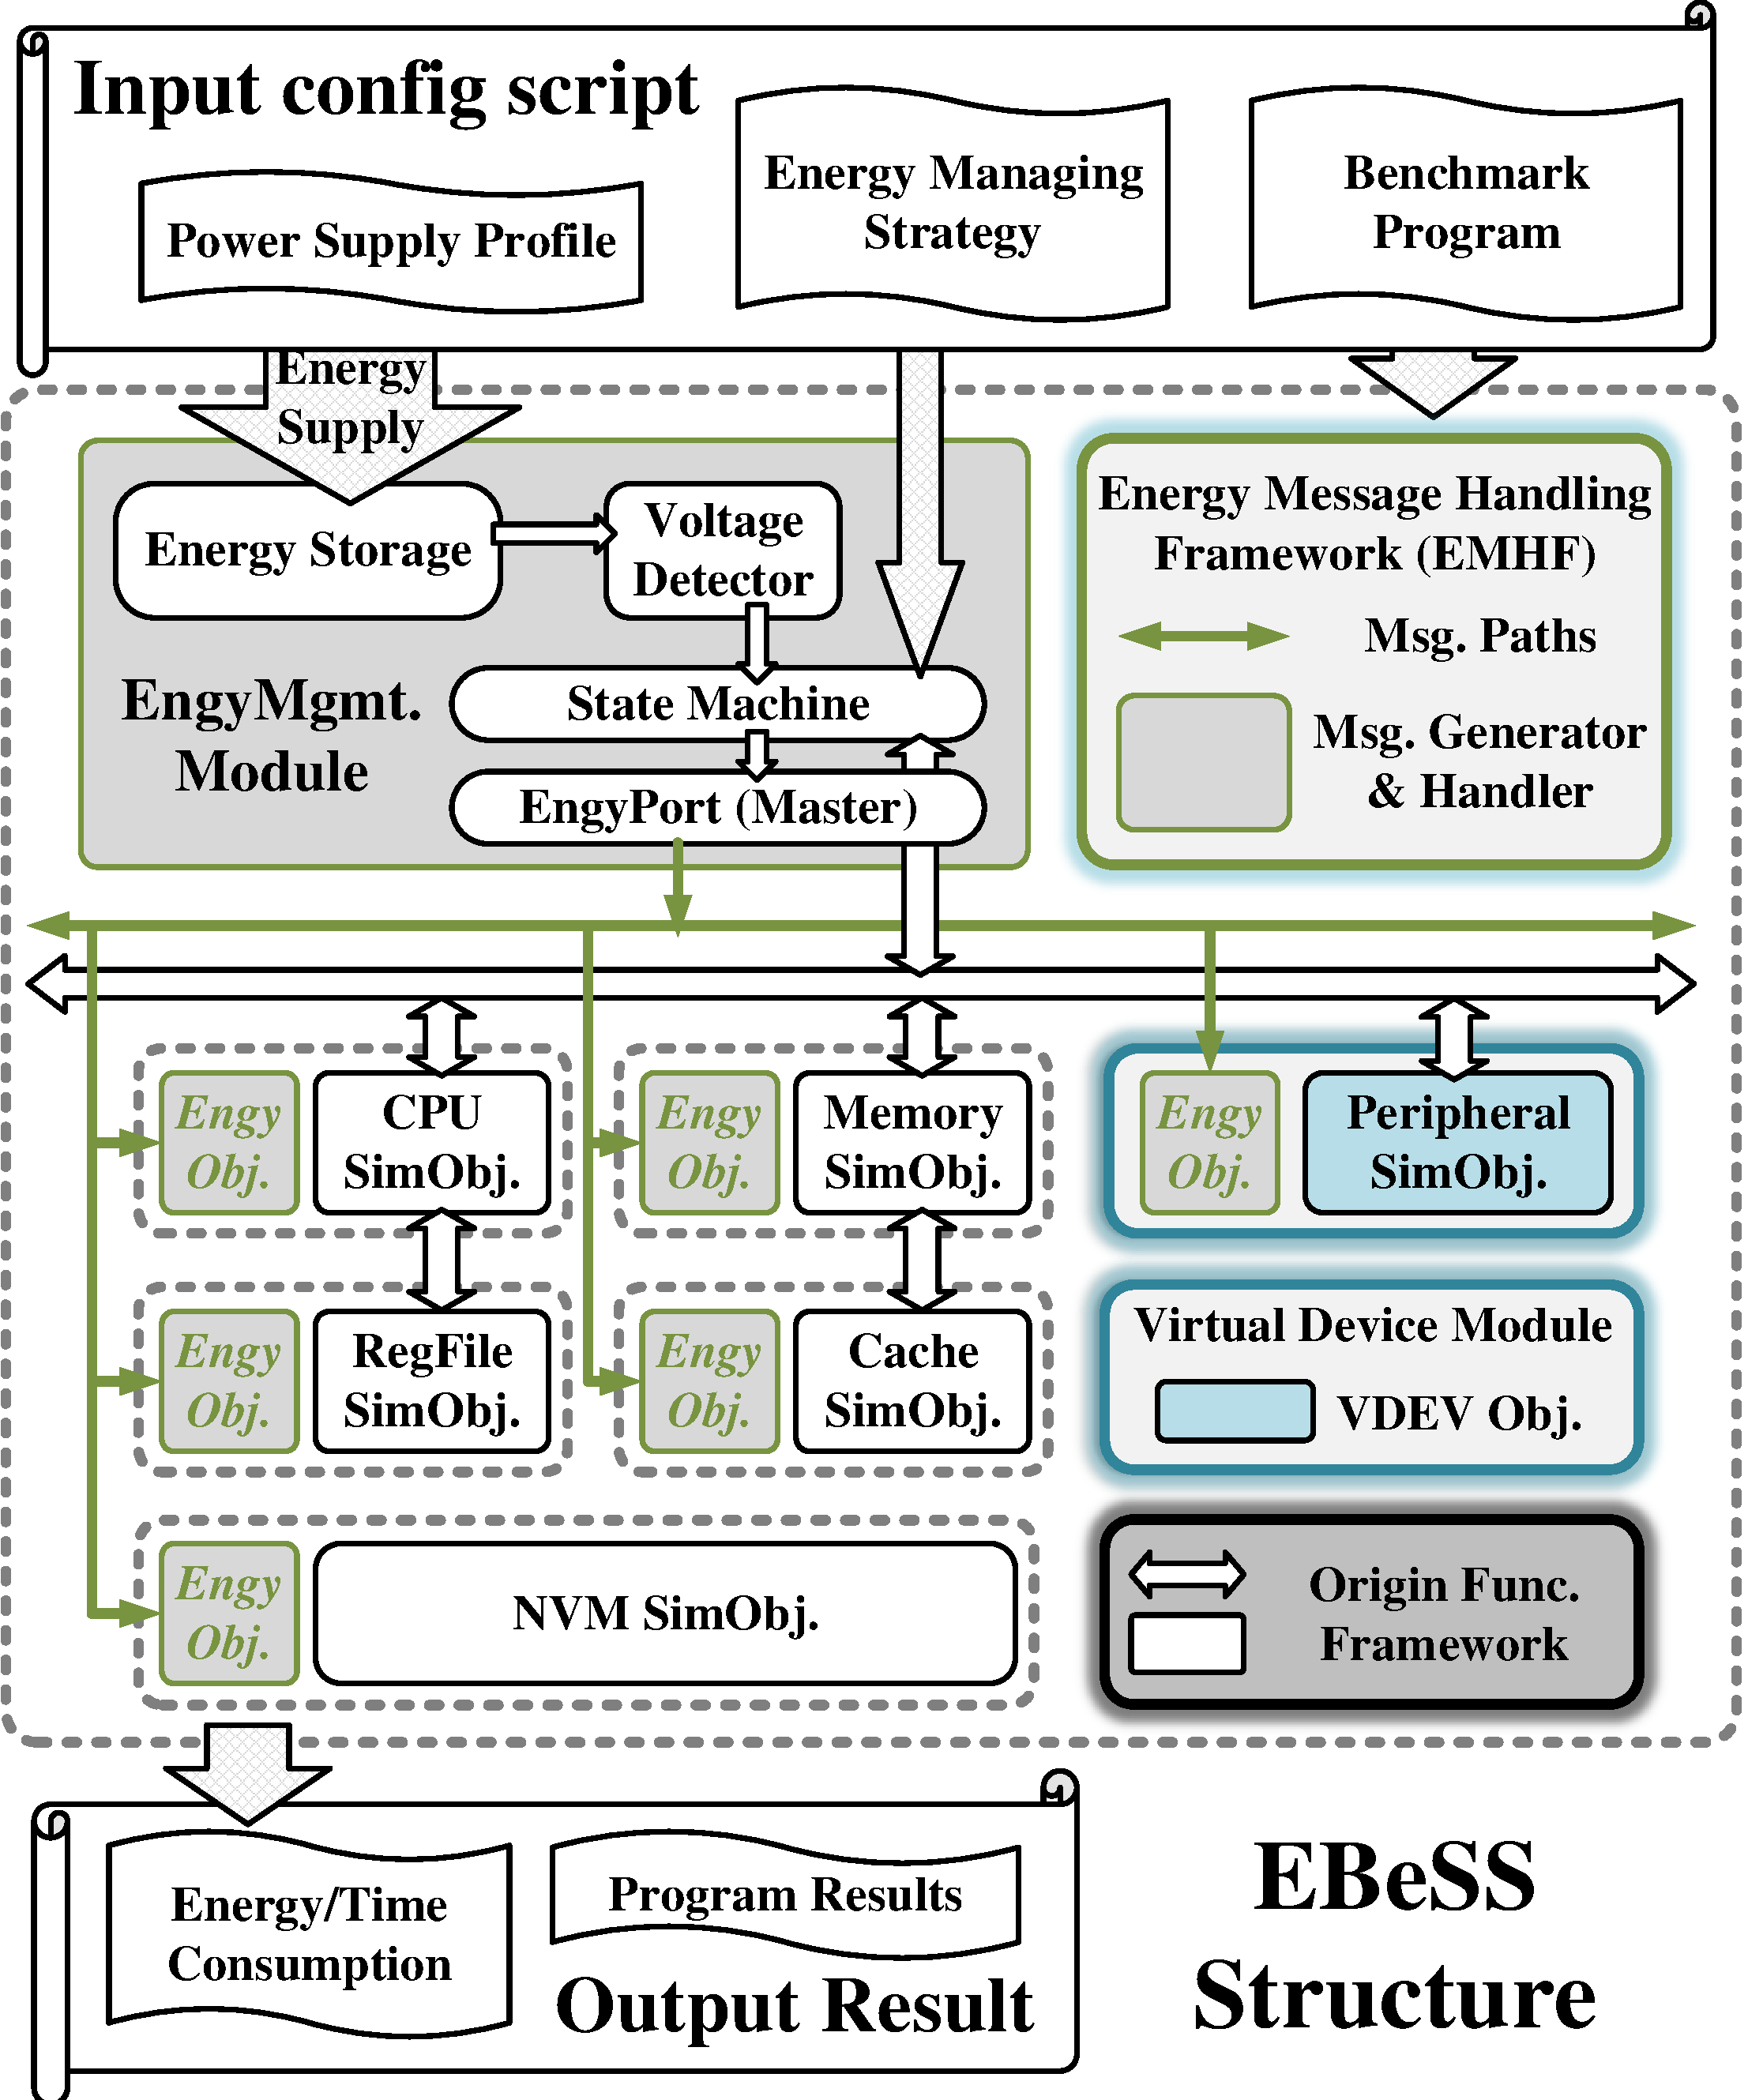
\includegraphics[width=0.5\textwidth]{EBeSS_Structure}
	\vspace{-20pt}
	\caption{Simulator structure of EBeSS. Two new components are added based on original GEM5 architecture. The energy message handling framework generates and handles the energy messages according to current energy conditions. The virtual device module creates an programmable object that supports the execution and energy behaviors of off-chip peripherals.}		\label{fig:techStructure}
\end{figure}

Energy Message Handling Framework allows the modules to have energy behaviors defined by energy management strategies when energy condition changes.
The framework reconstructs all the hardware modules in GEM5 with a new energy supported class, EnergyObject. 
With the help of EnergyObject, an energy management module (EMM) is designed to alarm the energy messages to other modules when the supply voltage changes.
According to the energy messages, each module, including CPU, memory and peripherals, takes actions defined by energy management strategies.
Details of the energy message handling framework is discussed in Sec.~\ref{sec:tech-EMHF}.

%
Virtual Device Module is an object that defines the connections and behaviors of off-chip peripherals which is vacant in the architecture of GEM5.
In this object, a memory mapping scheme is introduced to realize the fundamental operations, including peripheral reads/writes and interrupts.
In this way, virtual device module provides an easy way to simulate a system containing both CPU and peripherals.
Details of the virtual device module is discussed in Sec.~\ref{sec:tech-vdev}.

%
Power failure introduces new conditions where the behaviors of hardware modules are not addressed by current simulators.
When power outages take place, the system loses all the volatile states and data.
When the power is enough, a recover scheme is required to resume the entire system.
EBeSS develops energy behavior prototypes for these hardware modules.
A baseline recover scheme, \emph{2-thres}, is designed and implemented in EBeSS to support the recovery of CPU as well as the peripherals.
Implementation of 2-thres is given in Sec.~\ref{sec:tech-example}.


\subsection{Energy Message Handling Framework}	\label{sec:tech-EMHF}
% Overview
Energy message handling framework is used to monitor the power supply changes and trigger the energy behaviors of hardware modules.
In the framework, EnergyObject is designed as a parent class of all the hardware objects to defined their energy related behaviors. 
The structure of the EnergyObject is shown in Fig.~\ref{fig:EngyMsgFrameworkStructure} (a), which contains an energy port and an energy message handler.
The energy port is used to connect different EnergyObjects to create an energy message network.
The energy message handler is a programmable virtual function that defines the reactions of each hardware module when the power supply changes.
With the help of these two parts, EnergyObject allows the hardware modules to realize energy related behaviors, such as energy harvesting, consuming and energy message exchanges.

With the help of EnergyObject, EBeSS constructs the energy message handling framework with three components: the connector, the informer and the reactor, as shown in Fig.~\ref{fig:EngyMsgFrameworkStructure} (b).
The connector is used to create interconnections between the EnergyObjects and manage the energy message transmissions.
The informer converts the energy supply information into energy messages and broadcasts to overall the system.
The reactor is loaded in each EnergyObject to adjust the execution status according to the messages.
Both the informer and the reactor are EnergyObjects that contains different ports and handlers.
All these components are programmable for users to defined specific self-powered systems.

\begin{figure}[!htpb]
	\centering
	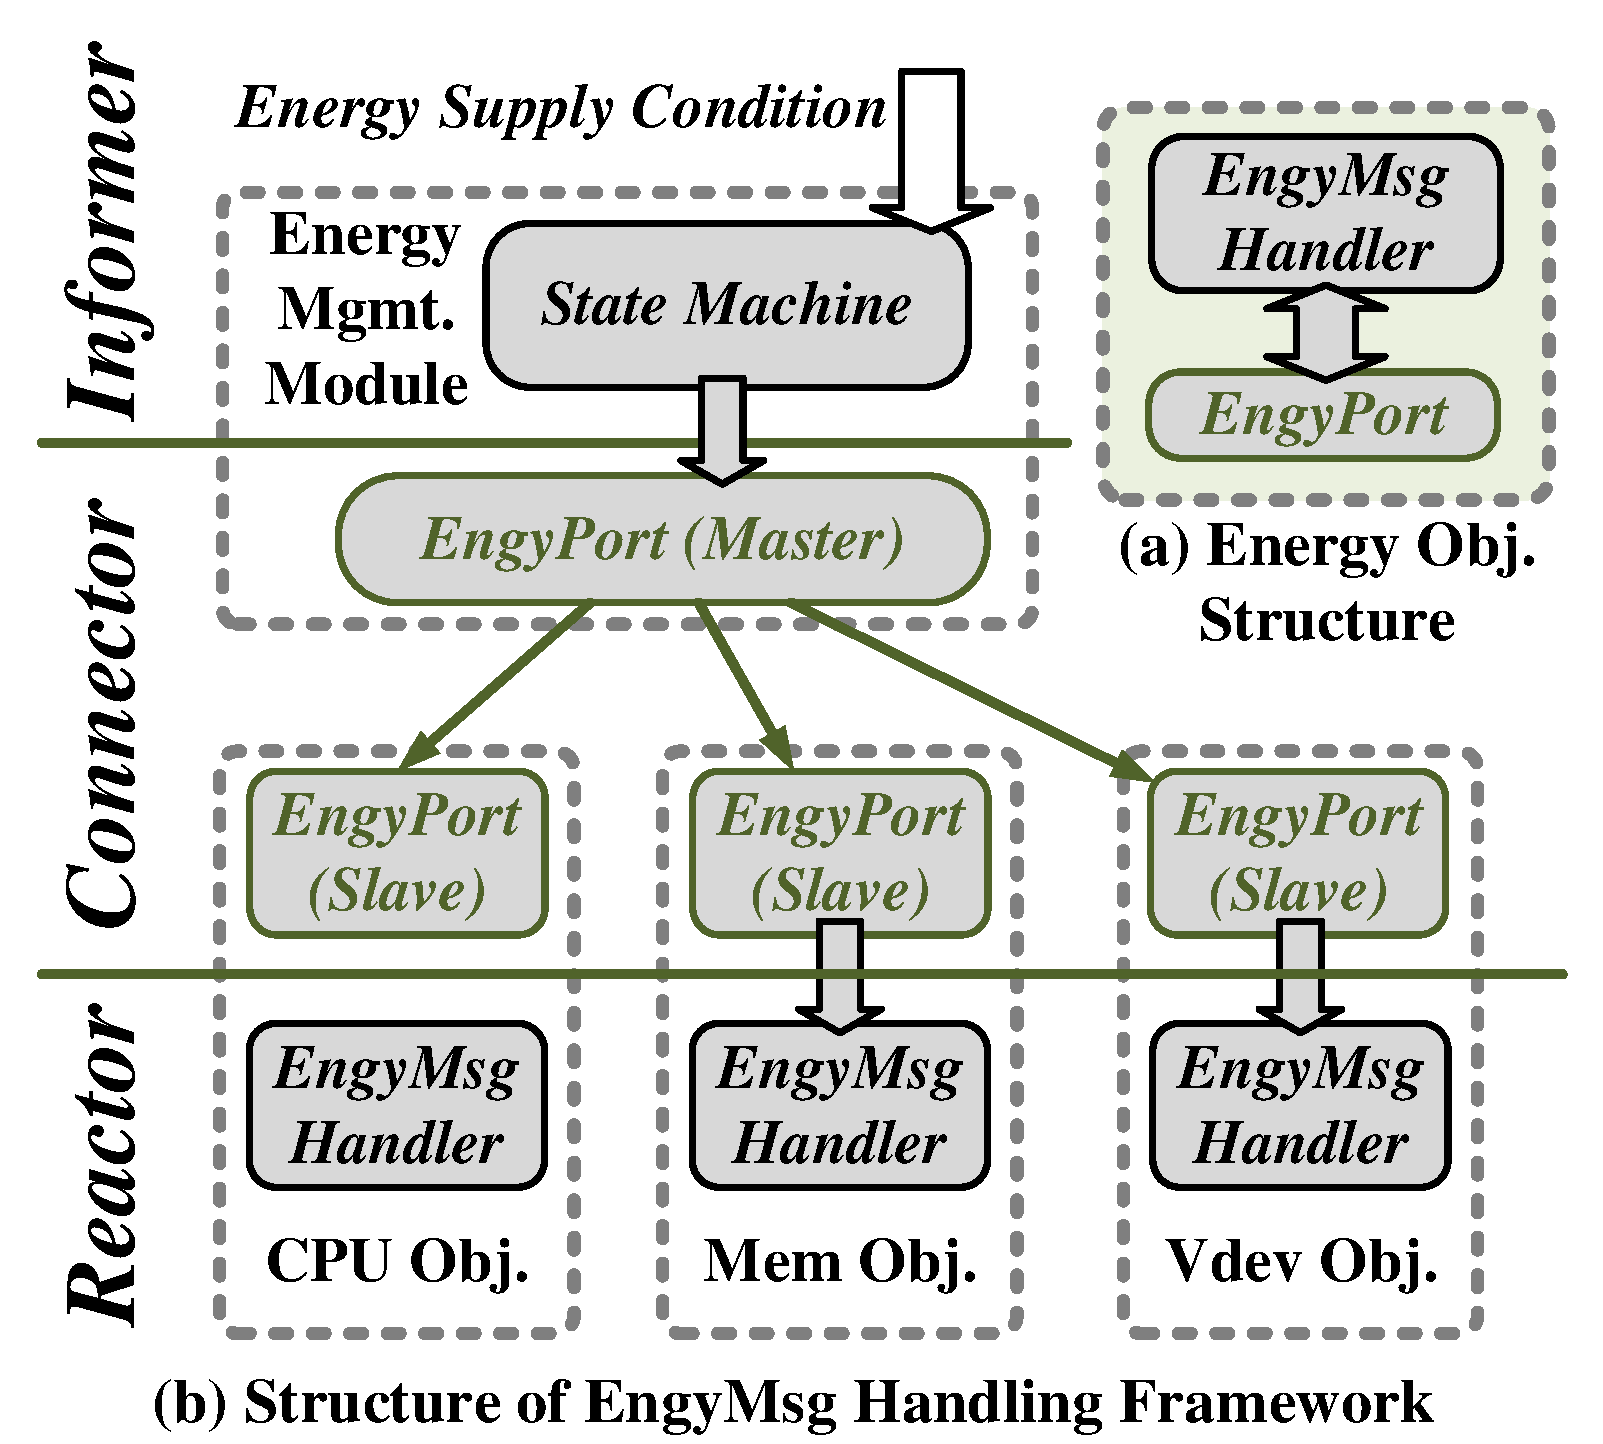
\includegraphics[width=0.45\textwidth]{EngyMsgFrameworkStructure}
	\vspace{-5pt}
	\caption{Structure of the energy message handling framework. The framework contains three components, the informer, the connector and the reactor.}		\label{fig:EngyMsgFrameworkStructure}
	\vspace{-15pt}
\end{figure}

\textbf{Connector: The Energy Port.\ \ }
% Energy Port
Energy Port is an interface that connects the EnergyObjects and exchanges the energy messages.
Each EnergyObject is connected to a specific energy port.
There are two types of energy ports: master ports and slave ports.
Master ports can actively broadcast energy messages and the slave ports passively accept and reply the energy consuming message and the execution status of their local hardware modules.
Master ports can only be connected to slave ports, and vice versa. 
Each master port can access multiple slaves and maintain a list of its slaves when a simulation is running, while a slave port can only track its unique master. 
The connections between those ports are established by users with simulation configuration profiles.

\textbf{Informer: Energy Management Module (EMM).\ \ }
% EMM
In the energy message handling framework, a user-defined object, EMM, is used as the informer to monitor the energy supply condition and broadcast energy messages.
In current NVP based energy harvesting systems, EMM is responsible to trigger energy behaviors, like power-on, power-off and voltage/frequency-changes, of each hardware module.
EMM adopts a state-machine and is connected to a master energy port to generate and broadcast energy messages.

\begin{figure}[!htpb]
	\centering
	\vspace{-5pt}
	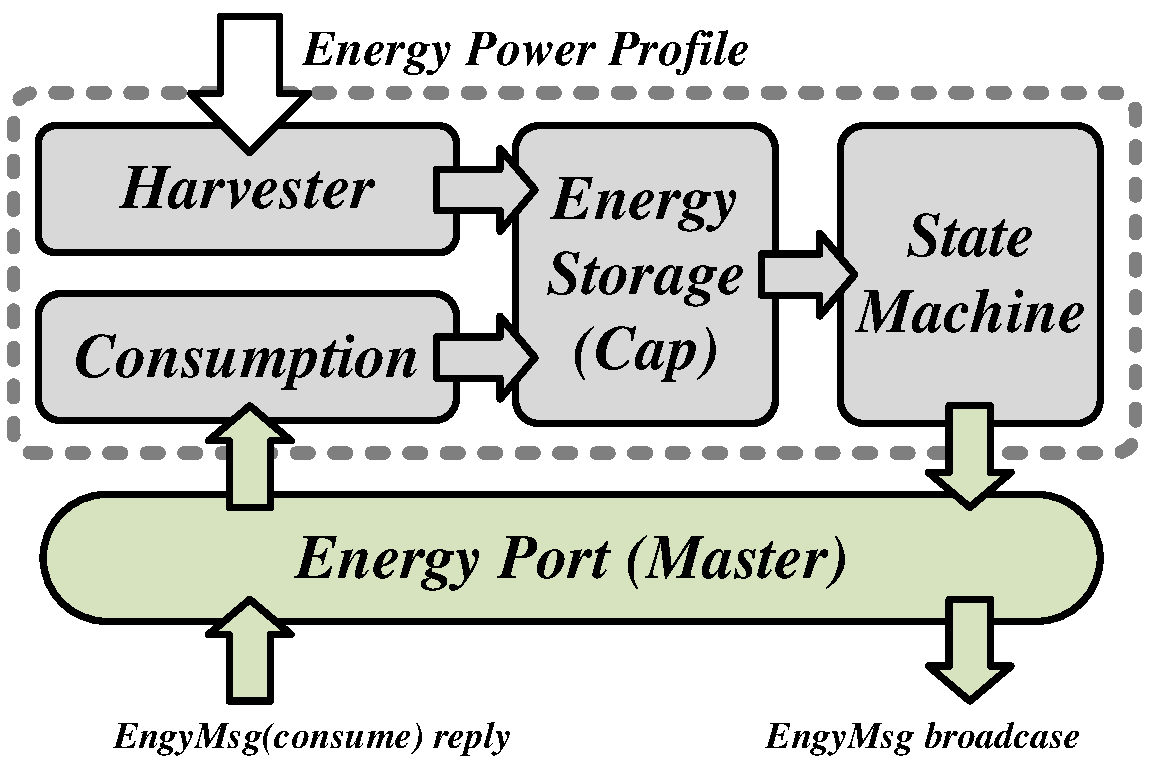
\includegraphics[width=0.35\textwidth]{EnergyManagementModule}
	\vspace{-10pt}
	\caption{The Structure and work flow of the energy Management Module.}		\label{fig:EnergyManagementModule}
\end{figure}

The structure and work flow of EMM is shown in Fig.~\ref{fig:EnergyManagementModule}.
After each time unit, the energy collection and consumption are committed to the energy storage (capacitors) and the current supply voltage is updated.
The income energy is harvested from an input energy profile and the energy consumption messages are received from other hardware modules.
When the supply voltage reaches certain thresholds, the energy state machine determines the state conversion and EMM broadcast energy messages via the master port to trigger energy behaviors of other modules.
To explore the optimal design of EMM algorithms and define more efficient and reliable energy behaviors, the energy harvesting part and the state machine are designed as pluggable functions in EMM.
%Users can define the behavior of energy harvest and state control by plugging custom modules into EnergyMgmt.

\textbf{Reactor: The Energy Message Handler.\ \ }
% Energy Reactor
Except for EMM, all the other modules are defined as reactors.
These modules are inherited from the EnergyObject, which connects to a slave energy port that receives and replies the upcoming energy messages and adopts an energy message handler to adjust the run-time execution states.
The message handler is used to define the energy behaviors.
According to design needs, users can modify the run-time states and data, such as execution states, reaction delay, reaction energy consumption and inner register data.
After the reaction, the reactor should reply its energy consumption as well as its execution status in a specific energy consuming message format to EMM to commit the energy costs.
Furthermore, EBeSS will open more authorities that the reactor replying more kinds of energy messages under the premise of system robustness.

\subsection{Virtual Device Module}	\label{sec:tech-vdev}
%
Although GEM5 provides powerful simulation ability to estimate the execution of the processor and memories, supports are still vacant for the off-chip peripherals, which play indispensable roles in energy harvesting systems.
Therefore, virtual devices are introduced into EBeSS to simulate the behavior of the volatile peripherals in energy harvesting systems.
Virtual device is a kind of memory-like module that CPU can simply make a request by accessing the address of a virtual device.
However, handling the address mapping of the virtual devices requires the support of an operating system which is not exist in a simple energy harvesting system (or SE mode of Gem5).
To fix the problem, EBeSS allows virtual devices to register virtual addresses in configuration files. 
When the CPU access a registered virtual address, the system will forward this access to the physical address of the related virtual device.
The address of virtual devices consists of 2 bytes as shown in Fig.~\ref{fig:VirtualDeviceAddress}.
The first byte is a control byte with control signals and the last byte constructs a 512B internal memory. 
In the control byte, four bits are used to control the executing status of the peripherals.
\emph{addr4} represents the correctness of the current peripheral task.
addr5 and addr6 show the status whether the peripheral is ready to be accessed.
addr7 is a configurable bit set by CPU to make a request to the virtual devices.

\begin{figure}[!htpb]
	\centering
	\vspace{-5pt}
	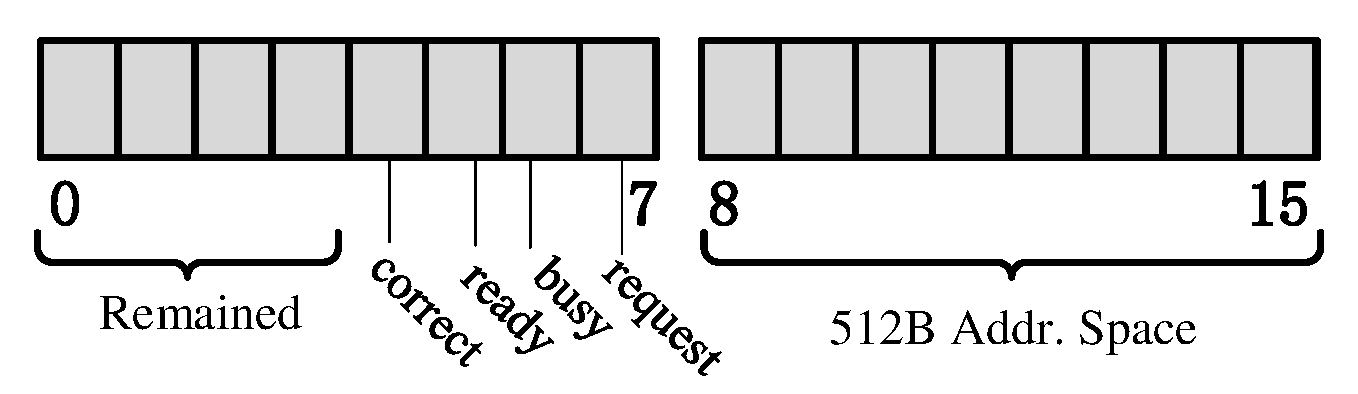
\includegraphics[width=0.4\textwidth]{VirtualDeviceAddress}
	\vspace{-5pt}
	\caption{The bit-level explanation of virtual device address definition.}	\label{fig:VirtualDeviceAddress}
\end{figure}

\subsection{Implementation of A Simple System Energy Behavior}	\label{sec:tech-example}
% 
Based on the architecture of EBeSS, we implement a baseline energy behavior strategy, \emph{2-thres}, based on the recover module in NVPSim~\cite{gu2016nvpsim}. 
The entire system consists of an EMM executing the 2-thres algorithm, a fully nonvolatile simple atomic NVP, a nonvolatile memory and volatile peripherals (virtual devices).
In these modules, the behavior of the NVM is omitted because power outages will not affect its states.

%
2-thres is an energy management method with a power-on threshold ($V_\text{on}$) and a power-off threshold ($V_\text{off}$).
When the supply voltage grows above $V_\text{on}$, a \emph{power-on} message is broadcast to the system and all the modules start/restarts.
When the supply voltage falls below $V_\text{off}$, a \emph{power-off} message is broadcast to the system and all the modules are shut down.

%
A fully nonvolatile simple atomic NVP is defined to match the 2-thres strategy.
NVP will save all the states to nonvolatile memories when power failure takes place.
In other words, the system pauses by consuming certain amount of energy after a certain time delay.
%The system has two states, on and off, and two energy messages are defined.
When power-off message arrives, the handler replies with the energy consumption of the backup operation and submit the backup delay to the event queue of GEM5.
Then EMM will update the energy storage voltage with the energy consumption and GEM5 will deschedule the events to pause the queue by inserting the backup delay.
Similarly, when power-on message arrives, the handler replies  the energy consumption of the restore operation and submit the restore delay.

\begin{figure}[!htpb]
	\centering
	\vspace{-5pt}
	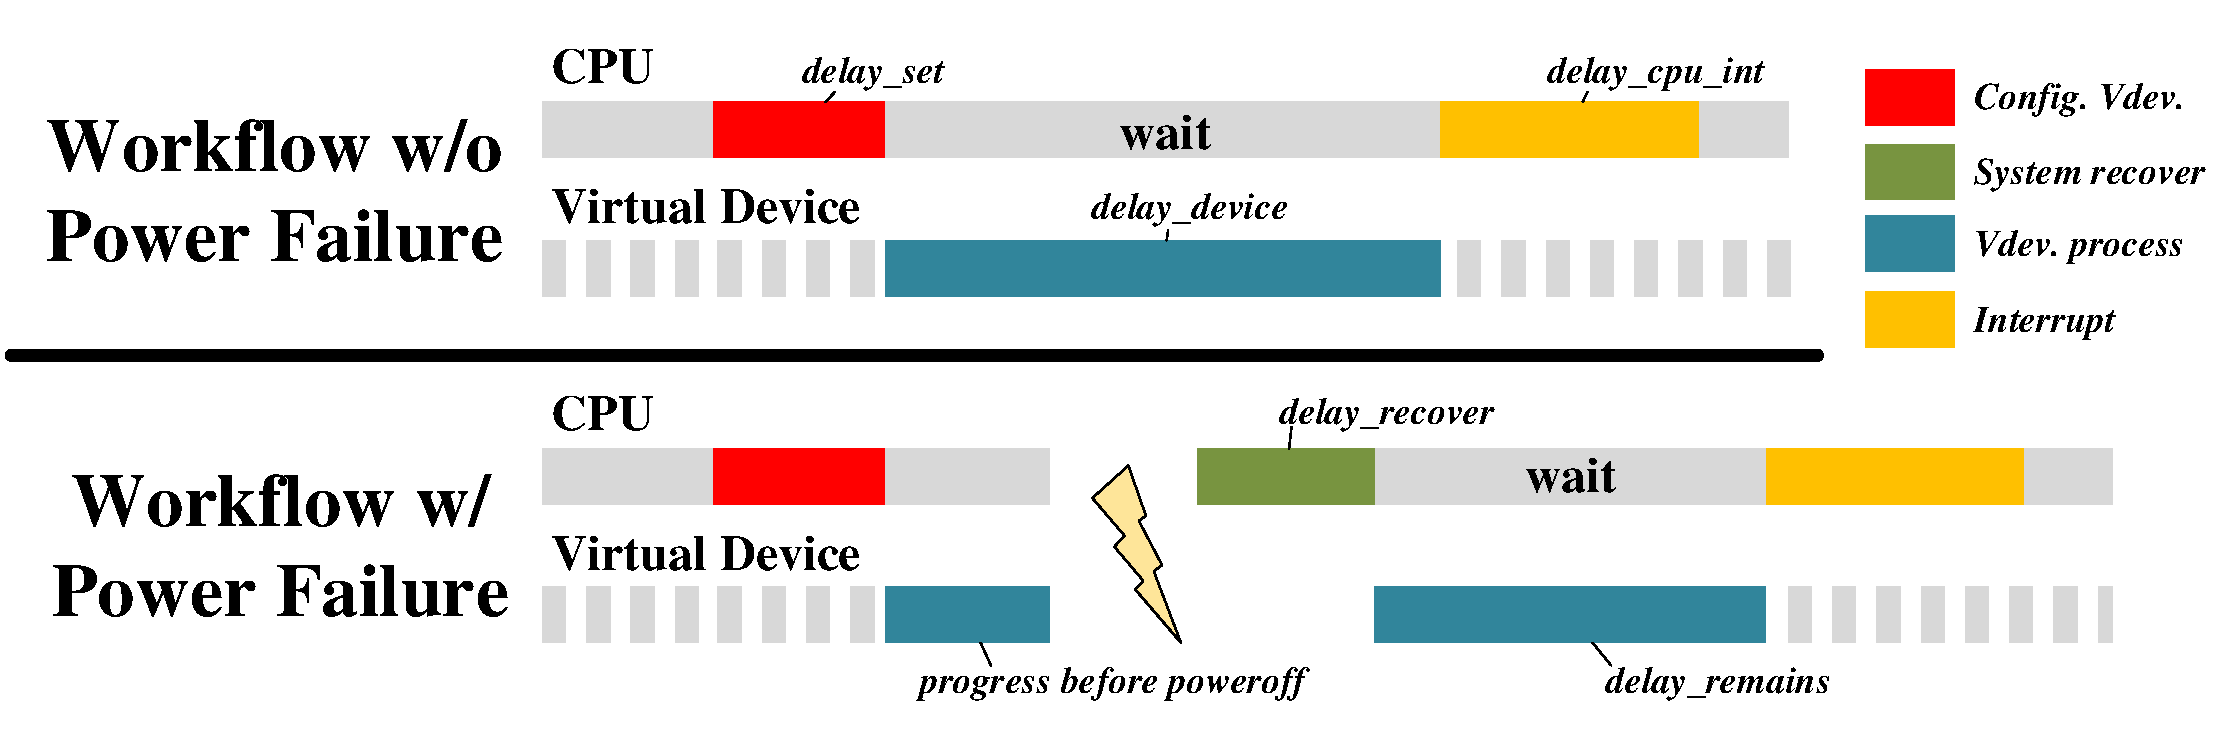
\includegraphics[width=0.5\textwidth]{VirtualDeviceBehavior}
	\vspace{-15pt}
	\caption{The work flow of virtual devices w and w/o power failures.}	\label{fig:VirtualDeviceBehavior}
\end{figure}

% Virtual Devices
The work mode of the virtual devices is shown in Fig.~\ref{fig:VirtualDeviceBehavior}.
In a normal execution without power failures, the entire work flow contains three stages.
First, NVP spends cycles (deley\_set) to set up the configurations of a virtual device.
Then, the virtual device executes a parallel task (delay\_device) and triggers an interrupt request for NVP to reply the execution results (delay\_cpu\_int).
The energy consumption of virtual device in each stage are committed to EMM.
When power failure takes place, most of the existing peripherals, such as sensors and transmitters, will lose its volatile states.
EBeSS pre-defines an ideal virtual device recovering model that the device can safely keep on the progress after a certain recover procedure (delay\_recover) which is executed by NVP.
